% !TEX encoding = UTF-8
% !TEX TS-program = pdflatex
% !TEX root = ../tesi.tex

%**************************************************************
\chapter{Progetto di stage}
\label{cap:progetto-di-stage}
%**************************************************************


%**************************************************************
\section{Lo stage per San Marco Group}

Il concetto di \textit{stage} formativo è molto importante per l'azienda San Marco Group. 
In primo luogo, viene considerata la sperimentazione di nuove tecnologie ed il loro confronto con quelle utilizzate quotidianamente. Per poterlo fare attualmente il personale presente dovrebbe smettere di svolgere le proprie attività, per questo motivo uno stagista universitario diventa una risorsa indispensabile, permettendo quindi all'azienda di sperimentare senza che vengano bloccate le normali mansioni.
Ci sono diverse realtà all'interno dell'azienda che possono considerarsi formative per uno studente e che attuano costantemente questa collaborazione:
\begin{itemize}
	\item \textbf{l'ufficio Risorse Umane}, offre a studenti del settore giuridico ed umanistico la possibilità di formarsi dal punto di vista professionale e personale grazie al vasto gruppo eterogeneo di personale presente in azienda; 
	\item \textbf{l'ufficio \textit{Marketing}}, molto sviluppato nell'azienda che dà spazio a figure che hanno intrapreso studi in ambito grafico o orientati alla comunicazione e al \textit{marketing web};
	\item \textbf{il laboratorio di Ricerca e Sviluppo}, la sezione, presente nella sede di Marcon, affianca studenti del settore chimico ad un gruppo di chimici \textit{senior} che svolge attività di studio e di ricerca su pitture decorative e decorativi per pavimenti, prodotti per le facciate, rivestimenti e sistemi termoisolanti; 
	\item \textbf{i \textit{Back office}}, che comprendono l'ufficio Acquisti e l'ufficio Commerciale, dove studenti del settore economico e commerciale hanno modo di confrontarsi con una realtà molto sviluppata e affermata nel territorio.
\end{itemize}
In secondo luogo, l'instaurazione del rapporto con l'Università di Padova è dato dalla possibilità di inserimento nell'azienda di risorse derivanti dal mondo accademico che, con una nuova prospettiva data dalle conoscenze apprese e messe in pratica nel corso di studio, possono portare idee creative e innovative, dalle quali può trarre beneficio anche il personale aziendale.

%**************************************************************
\section{Contesto attuale}

Attualmente l'azienda è nel vivo di un progetto di cambio gestionale, motivato principalmente da:
\begin{itemize}
	\item la fine del supporto tecnico da parte di \textit{Microsoft} sul gestionale attualmente adottato (\textit{Microsoft Dynamics Ax 2009}, figura \ref{fig:ax-2009}) fissato per il 12 ottobre 2021;
	\item insoddisfazione da parte della direzione sul prodotto.
\end{itemize}
Esisteva la possibilità di continuare ad utilizzare la versione 2009 anche oltre alla fine del supporto, affidandosi ad un partner terzo per la manutenzione e le implementazioni dei vari adeguamenti necessari a soddisfare periodicamente le regole stabilite nel contesto fiscale. Questa scelta però è stata ritenuta troppo rischiosa perché, in caso di inadempienze del partner scelto, ci sarebbero potute essere delle conseguenze importanti per l'azienda, come ad esempio l'impossibilità di adempiere agli obblighi fiscali.
Si è deciso quindi di cambiare il \textit{software}.\\
E' stata effettuata l'analisi da parte di un'azienda di consulenza di tutti i processi aziendali, così da individuarne le criticità: in questo modo il cambio di \textit{software} gestionale non avrebbe solamente soddisfatto le necessità ma anche apportato un miglioramento. Successivamente è iniziata la \textit{software selection}.

\vspace{10pt}
\begin{figure}[htbp]
	\begin{center}
		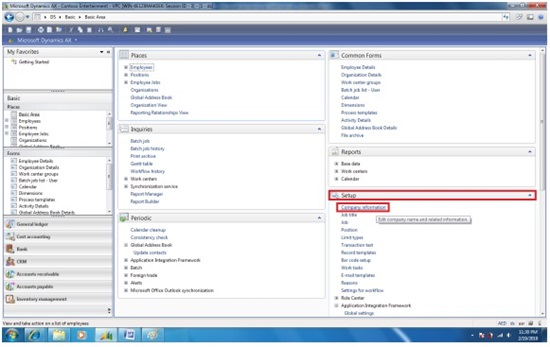
\includegraphics[height=8cm]{ax-2009}
		\caption{Interfaccia utente \textit{Microsoft Dynamics Ax 2009}. \newline \textbf{Fonte: }\url{https://community.dynamics.com/}}
		\label{fig:ax-2009}
	\end{center}
\end{figure}
\vspace{10pt}

Tra i vari \textit{software} gestionali presenti sul mercato, è stato preso in considerazione \textit{Microsoft Dynamics 365}. La nuova versione dell'\textit{ERP} di \textit{Microsoft} differisce in maniera sostanziale da quella attualmente utilizzata, principalmente per quanto riguarda:
\begin{itemize}
	\item la re-ingegnerizzazione della base di dati, che richiederebbe una reimpostazione radicale della base di dati attuale;
	\item la dismissione del modello di sviluppo a \textit{layer}, che consiste nell'utilizzo di una gerarchia di livelli nei quali vengono implementati i metodi degli elementi applicativi presenti nel gestionale. Quando viene eseguito un metodo di un qualsiasi elemento applicativo, il sistema parte dal \textit{layer} più esterno per verificare ed eseguire, se disponibile, un'implementazione del metodo per quell'elemento, altrimenti si sposta sul \textit{layer} più interno per ripetere l'operazione fino ad arrivare al \textit{layer} di sistema.In questo modo è possibile personalizzare facilmente le varie funzionalità presenti, attività che con la nuova versione richiederebbero un processo più impegnativo.
\end{itemize}
L'adozione di \textit{Microsoft Dynamics 365} sarebbe stata troppo impegnativa dal punto di vista tecnico sia nel breve che nel lungo termine, per questo motivo è stato scartato.
Alla fine della valutazione la scelta è ricaduta su \textit{Sage X3}, per la sua adattabilità e perché rispecchia maggiormente le necessità aziendali; è perciò iniziata la fase di implementazione del nuovo \textit{software} attraverso:

\begin{itemize}
	\item sviluppi per adeguamento delle funzionalità del nuovo gestionale agli\textit{ standard} aziendali;
	\item migrazione dei dati;
	\item formazione degli utenti finali.
\end{itemize}

Di seguito vediamo un'immagine riassuntiva sulle tecnologie che compongono il software gestionale e un'accenno alla sua architettura di sistema, descritta più in dettaglio in \ref{cap:architettura-sage}.

\vspace{10pt}
\begin{figure}[htbp]
	\begin{center}
		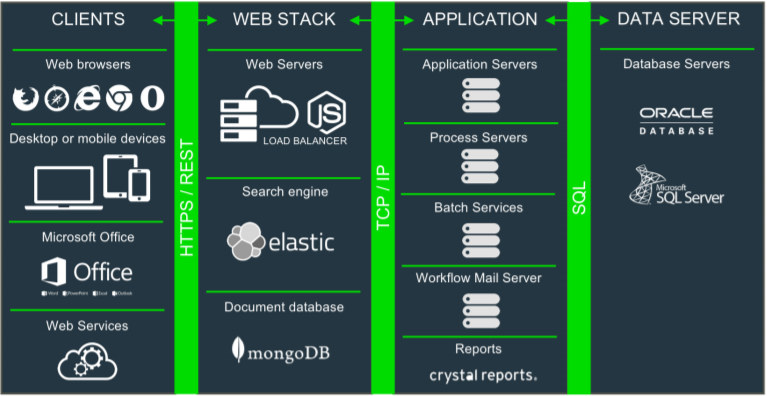
\includegraphics[height=7cm]{sage-x3}
		\caption{Architettura di sistema di \textit{Sage X3}. \newline \textbf{Fonte:}\url{https://partnerportal.sagex3.com/}}
	\end{center}
\end{figure}
\vspace{30pt}


%**************************************************************
\section{Proposta di stage}

Lo scopo dello \textit{stage} consisteva nello sviluppo \textit{software} di un sistema di gestione di offerte di fornitura, dedicate a beni materiali e servizi. Dopo l'analisi del processo, il mio compito era quello di sviluppare un'applicazione \textit{web} che permettesse agli utenti interni la gestione delle richieste e ai fornitori designati di rispondere con delle proposte di offerta.
L'applicazione da sviluppare doveva avere le seguenti caratteristiche:
\begin{itemize}
	\item capacità di interfaccia con il database del gestionale tramite \textit{web service};
	\item la sezione destinata alle richieste di servizio di trasporto doveva rispettare il layout del modulo cartaceo utilizzato;
\end{itemize}

Inoltre avevo il compito di redigere un \textit{report} con il dettaglio della richiesta e in base al tempo disponibile, fornire delle statistiche sulla base dei dati utilizzati.\\ Quest'ultimi sarebbero stati utili all'analisi di \textit{BI} in un' ottica di miglioramento del processo aziendale.


\subsection{Prodotti attesi}
L'attività di \textit{stage} prevedeva la produzione dei seguenti oggetti, documenti e \textit{software}:
\begin{itemize}
	\item relazione sul processo aziendale coinvolto;
	\item relazione sulla progettazione architetturale;
	\item codice sorgente dell'applicazione \textit{web};
	\item manuale e documentazione riguardante la struttura dell'applicazione \textit{web} per	manutenzione ed eventuali integrazioni;
	\item \textit{report} di dettaglio dell'offerta;
	\item \textit{report} con statistiche utili all'analisi di \textit{BI}.
\end{itemize}


\subsection{Priorità e obiettivi dello stage}
Per identificare gli obiettivi ed il loro livello di priorità, ho associato a ciascuno di essi un codice nel formato sottostante:
\\
\begin{center}
	\textit{<obiettivo.[sotto-obiettivo]-tipologia>. }
\end{center}

Il significato del codice è il seguente:
\begin{itemize}
\item \textbf{obiettivo}, indica il numero univoco dell'obiettivo;
\item \textbf{sotto-obiettivo}, è il numero univoco del sotto-obiettivo, ed è opzionale, essendo riportato solo nel caso in cui l'obiettivo sia suddiviso in sotto-obiettivi;
\item \textbf{tipologia}, indica il livello di priorità assegnato all'obiettivo.
\end{itemize}
La tipologia determina l'importanza di realizzare tale obiettivo, ed è scelta tra le seguenti:
\begin{itemize}
	\item \textbf{OB}, indica un obiettivo obbligatorio, il cui raggiungimento è necessario;
	\item \textbf{DE}, indica un obiettivo desiderabile, il cui raggiungimento è importante e dal riconoscibile valore aggiunto, ma non necessario.
\end{itemize}

\newpage

\begin{center}
	\begin{longtable}{|c|c|}
		\caption{Tabella riassuntiva degli gli obiettivi dello \textit{stage}.}\\
		\hline
		\textbf{Obiettivo} & \textbf{Descrizione}\\
		\hline
		1-OB & Comprensione del problema\\
		\hline
		2-OB & Comprensione delle tecnologie di \textit{backend}\\
		\hline
		2.1-OB & Comprensione di \textit{Sage X3}\\
		\hline
		2.2-OB & Comprensione del database \textit{SQL Server}\\
		\hline
		2.3-OB & Comprensione della tecnologia dei \textit{web service}\\
		\hline
		3-OB & Comprensione delle tecnologie di \textit{frontend}\\
		\hline
		3.1-OB & Comprensione di \textit{Javascript}\\
		\hline
		3.2-OB & Comprensione di \textit{jQuery}\\
		\hline
		4-OB & Sviluppo dell'applicazione \textit{web}\\
		\hline
		5-OB & Sviluppo del \textit{report} di dettaglio della richiesta\\
		\hline
		6-OB & Validazione del prodotto\\
		\hline
		7-DE & Sviluppo del \textit{report} con le statistiche utili all'analisi \textit{BI}\\
		\hline
	\end{longtable}
\end{center}


\subsection{Vincoli}
\subsubsection{Vincoli temporali e organizzativi}
Il progetto di \textit{stage} ha avuto una durata di 320 ore, distribuite nell'arco di tre mesi, con settimane lavorative di 25 ore ciascuna.
In accordo con il relatore e il \textit{tutor} aziendale, lo \textit{stage} è stato svolto prevalentemente in modalità \textit{smart working}.
Con lo scopo di informare il mio relatore  dei progressi, ogni 5 giorni lavorativi dovevo provvedere a inviare un resoconto dello stato di avanzamento rispetto alle attese del piano di lavoro e ad eventuali deviazioni da esso.\\Invece, con il \textit{tutor} aziendale, avevo previsto almeno un incontro a settimana in remoto o fisicamente in azienda per discutere del progresso e di eventuali cambiamenti da apportare al progetto.
\subsubsection{Vincoli tecnologici}
Lo sviluppo del progetto prevedeva alcuni vincoli imposti dall'azienda.
In primo luogo l'utilizzo della tecnologia \textit{SOAP}, \textit{Simple Object Access Protocol}, per i \textit{web service} che permettevano l'interfacciamento tra l'applicazione \textit{web} e il gestionale.
In secondo luogo, l'utilizzo dello strumento per la produzione di stampe di dati \textit{Crystal Reports} per produrre il \textit{report} di dettaglio della richiesta d'offerta e il \textit{report} con le statistiche utili all'analisi della \textit{BI}.


\subsection{Pianificazione}

Il Piano di Lavoro, redatto insieme al \textit{tutor} aziendale, prevedeva inizialmente 4 fasi, ognuna delle quali della durata di 3 settimane lavorative:
\begin{itemize}
	\item studio del processo aziendale e formazione sulle tecnologie coinvolte nello sviluppo dell'applicazione \textit{web} e dell'interfacciamento con il gestionale;
	\item progettazione della soluzione e configurazione dell'ambiente di sviluppo;
	\item realizzazione dell'applicazione \textit{web} e fase di \textit{testing};
	\item formazione sul \textit{software} per la produzione di stampe e sviluppo dei \textit{report};
\end{itemize}
L'ultima settimana di \textit{stage} prevedeva la verifica e la validazione finale.
Di seguito un dettaglio delle fasi appena descritte:

\begin{center}
	\begin{longtable}{|c|c|}
		\caption{Dettaglio pianificazione del progetto di \textit{stage}.}\\		
		\hline
		\textbf{Ore} & \textbf{Attività}\\
		\hline
		40 & Formazione sulle tecnologie\\
		\hline
		35 & Analisi del problema\\
		\hline
		25 & Stesura documentazione relativa ad analisi e progettazione\\
		\hline
		55 & Progettazione della soluzione\\
		\hline
		15 & Configurazione dell'ambiente di sviluppo\\
		\hline
		60 & Sviluppo dell'applicazione \textit{web}\\
		\hline
		20 & \textit{Test} sull'applicazione \textit{web}\\
		\hline
		25 & \textit{Test} sui \textit{web service}\\
		\hline
		25 & Formazione su strumento e produzione \textit{report}\\
		\hline
		5 & Stesura documentazione finale\\
		\hline
		15 & Verifica e validazione finale\\
		\hline
	\end{longtable}
\end{center}


%**************************************************************
\section{Analisi preventiva dei rischi}
Nella fase iniziale di analisi ho individuato alcuni possibili rischi in cui poter incorrere.\\
Successivamente, ho provveduto ad elaborare delle possibili soluzioni per far loro fronte.
\\
\begin{risk}{Tecnologie e \textit{framework} sconosciuti}
	\riskdescription{Durante lo svolgimento dello \textit{stage} era previsto l'utilizzo di tecnologie a me ancora sconosciute}
	\risksolution{Nella fase di pianificazione iniziale ho programmato un periodo di auto-formazione sulle tecnologie e sui \textit{framework} da utilizzare}	
\end{risk}
\begin{risk}{Incomprensioni sul processo aziendale}
	\riskdescription{A causa dei vari enti coinvolti nella fase di analisi e del gran numero di attività svolte attualmente extra sistema (utilizzo di moduli cartacei, contatti telefonici direttamente coi fornitori, ecc.), avevo previsto di non riuscire a delineare e comprendere pienamente il processo aziendale interessato}
	\risksolution{In accordo con il \textit{tutor} aziendale, sono stati individuati dei \textit{key users}, uno per ogni ufficio coinvolto, che si sono resi disponibili ad offrire un maggior dettaglio sulle fasi che interessano la loro attività}	
\end{risk}
\begin{risk}{Scelte non ottimali}
	\riskdescription{A causa dell'inesperienza avevo considerato l'idea di non riuscire a comprendere le attività da svolgere o di fare scelte non adeguate alle aspettative aziendali}
	\risksolution{Tutte le scelte progettuali fondamentali sono state discusse e supervisionate dal \textit{tutor} aziendale}
\end{risk}

%**************************************************************
\section{Motivazione della scelta}

\subsection{Motivazioni personali}

Una delle principali motivazioni che mi hanno portato a scegliere questa proposta di \textit{stage} curricolare, era il contesto di inserimento: volevo capire come una grande azienda, il cui settore di impiego non è strettamente legato a quello informatico, si approccia alle nuove tecnologie e si appoggia all'informatica per il suo business. 
\\
Il mio intento era di riuscire ad avere una visione d'insieme per capire quali attività vengono svolte per supportare un'azienda, non solo del contesto dello sviluppo \textit{software} ma anche nell'ausilio di altri processi.
\\
Inoltre, l'opportunità offertami dall'azienda non si sarebbe fermata al semplice \textit{stage} curricolare o all'assunzione per la sola occupazione lavorativa, ma quella che mi è stata proposta era allo stesso tempo la possibilità di supporto nel mio percorso di studi fornendomi un impiego retribuito, a riprova di una \textit{vision} contemporanea che vede negli stagisti non uno svantaggio, ma una risorsa che porta nuova linfa all'interno di un mondo lavorativo consolidato.
\\
A conclusione dello \textit{stage} mi attirava la possibilità di continuare a seguire le attività successive allo sviluppo del prodotto, come la formazione degli utenti, e vedere i risultati del mio lavoro nel lungo termine.

\subsection{Motivazioni professionali}

La mia scelta di \textit{stage} è ricaduta su questa azienda perché rispetto alle altre con cui ho avuto contatti grazie all'evento di incontro \textit{StageIt} in cui le principali aziende del territorio propongono i loro \textit{stage} formativi in ambito \textit{\gls{ict}\glsfirstoccur}, questa mi avrebbe offerto l'opportunità di vedere non solo da vicino il processo di sviluppo di un nuovo gestionale, ma di svilupparlo a diretto contatto con gli utenti finali e non solo come un servizio offerto dall'esterno (ad esempio un'azienda di sola consulenza informatica), esperienza molto più stimolante per chi alle prime armi si avvicina al mondo del lavoro.
\\
Mi interessava dunque il fatto di potermi rapportare direttamente con gli utenti finali del prodotto, in modo da poter comprendere meglio le problematiche che si possono incontrare in fase di analisi e riuscire ad applicare i concetti studiati nel corso di Ingegneria del Software. 
\\ 
Infine, essendo in pieno sviluppo un progetto di cambio gestionale, ho ritenuto fosse un'opportunità ad alto contenuto formativo, sia per le tecnologie utilizzate a me ancora sconosciute, sia per la possibilità di interfacciarmi e collaborare direttamente con figure professionali interne ed esterne all'azienda impegnate nel progetto.
